%%%%%%%%%%%%%%%%%%%%%%%%%%%%%%%%%%%%%%%%%%%%%%%%%%%%%%%%%%%%%%%%%%%%%%%%%%%%%%%%
%2345678901234567890123456789012345678901234567890123456789012345678901234567890
%        1         2         3         4         5         6         7         8

\documentclass[letterpaper, 10 pt, conference]{ieeeconf}  % Comment this line out if you need a4paper

%\documentclass[a4paper, 10pt, conference]{ieeeconf}      % Use this line for a4 paper

\IEEEoverridecommandlockouts                              % This command is only needed if 
                                                          % you want to use the \thanks command

\overrideIEEEmargins                                      % Needed to meet printer requirements.

%In case you encounter the following error:
%Error 1010 The PDF file may be corrupt (unable to open PDF file) OR
%Error 1000 An error occurred while parsing a contents stream. Unable to analyze the PDF file.
%This is a known problem with pdfLaTeX conversion filter. The file cannot be opened with acrobat reader
%Please use one of the alternatives below to circumvent this error by uncommenting one or the other
%\pdfobjcompresslevel=0
%\pdfminorversion=4

% See the \addtolength command later in the file to balance the column lengths
% on the last page of the document

% The following packages can be found on http:\\www.ctan.org
\usepackage{graphics} % for pdf, bitmapped graphics files
\usepackage{epsfig} % for postscript graphics files
\usepackage{mathptmx} % assumes new font selection scheme installed
\usepackage{mathtools}
\usepackage{times} % assumes new font selection scheme installed
\usepackage{mathrsfs}
\usepackage{amsmath} % assumes amsmath package installed
\usepackage{amssymb}  % assumes amsmath package installed
\usepackage{bm}
\usepackage{upgreek}
\usepackage{xcolor}
\usepackage{empheq}
\usepackage{IEEEtrantools}
\usepackage{subcaption} 


\newcommand{\R}{\ensuremath{\mathbb{R}}}
\usepackage[
%utf8,
linesnumbered,ruled,vlined]{algorithm2e}
\usepackage {algpseudocode}
\usepackage{algorithmicx}
\usepackage{algcompatible}

\title{\LARGE \bf
Performance Constrained Greedy Selection and Supermodular Approximation under Quadratic Observations
}

\author{Wooyeong Cho, Tengyou Xu, Kaden Bautista and Ankur Mehta$% <-this % stops a space
%\thanks{*This work was not supported by any organization}% <-this % stops a space
\thanks{Department of Electrical and Computer Engineering,
University of California Los Angeles, Los Angeles, CA, USA.
        {\tt\small {chowy1628,tengyoux,kadenbautista21,mehtank} @ucla.edu}}%
}

\begin{document}

\maketitle
\thispagestyle{empty}
\pagestyle{empty}


%[What specific problem are you addressing in particular]
%[What specific challenges are you addressing in this problem] 
%[What is your specific approach to solving this subproblem?]
%[How can you be reasonably sure this approach will result in a solution? with numbers]
%%%%%%%%%%%%%%%%%%%%%%%%%%%%%%%%%%%%%%%%%%%%%%%%%%%%%%%%%%%%%%%%%%%%%%%%%%%%%%%%
\begin{abstract}
We address the problem of selecting the smallest subset of measurements for nonlinear quadratic observation models subject to a target estimation-accuracy constraint. This problem is NP-hard, and under quadratic observations, the exact posterior covariance is generally intractable, limiting the direct estimation-error analysis and the applicability of existing greedy guarantees. To address these challenges, we propose a performance-constrained greedy measurement selection framework that employs a closed-form Van Trees surrogate, resulting in a non-supermodular objective. First, we establish a measurement-utilization guarantee that bounds the number of measurement selected by optimal solution relative to that of greedy solution. We also derive the first explicit, computable lower bound on the supermodularity ratio of the surrogate objective for observation models with nonzero linear terms and full-rank quadratic sensing matrices, a setting in which prior work establishes weak submodularity only qualitatively. Our numerical experiments demonstrate that the proposed method outperforms a linearized-model baseline in measurement use and that the proposed bound remains a valid conservative certificate across various model parameters.

\end{abstract}
%%%%%%%%%%%%%%%%%%%%%%%%%%%%%%%%%%%%%%%%%%%%%%%%%%%%%%%%%%%%%%%%%%%%%%%%%%%%%%%%
\section{INTRODUCTION}


%overall problem description[what is sensor scheduling], [Which industries mainly need this research?], [Why on earth are they doing this research?]
Optimal measurement selection is the problem of choosing a subset of available sensors or measurements to achieve a desired estimation or monitoring performance while considering practical resource constraints such as limited energy, communication bandwidth, and computation. This problem arises in many real-world systems, including autonomous robots \cite{c1,c2}, distributed sensor networks \cite{c3,c4}, intelligent transportation systems \cite{c5}, and surveillance or target-tracking applications \cite{c6,c7}, where large numbers of sensors are available but only a fraction can be activated efficiently at any given time. In such settings, continuously using every sensor is often costly or even infeasible. Consequently, the goal of optimal measurement selection is to identify the smallest or most informative subset of measurements that preserves the required performance while reducing overall resource usage.

%[One of main challenges in overall problem that I'm addressing ] 
A fundamental challenge in this problem is its combinatorial nature. As the number of available sensors increases, the number of possible measurement subsets grows exponentially, making exact optimization computationally intractable in practice. Existing work \cite{c8,c9,c10} has identified this combinatorial complexity as a central obstacle and has established theoretical limits as well as exact formulations for optimal selection.

%[What has been done so far to address this overall problem?(greedy and submodularity/supermodularity) and Why preivious existing research happened? How did they try to solve the problem?]
Because the problem is NP-hard \cite{c10,c11}, a major line of prior research has focused on identifying structural properties of the objective that enable efficient approximation algorithms. In particular, submodularity and supermodularity have played an important role in justifying greedy selection methods with provable performance guarantees \cite{c12,c13,c14}. Even when the objective does not satisfy these properties exactly, approximate or weak submodularity/supermodularity has been used to extend greedy guarantees to more general settings. For example, \cite{c15,c16} leverage weak supermodularity to analyze the minimization of non-submodular estimation metrics such as mean-square error. These works show that even when the objective does not exhibit exact diminishing returns, suitable constant-factor characterizations can still quantify its deviation from ideal structure and yield meaningful greedy performance guarantees.

%[What additional specific challenges are you addressing in this problem (sensor usage approximation under nonlinear model/quadratic observations)]
%Why preivious existing research(Hashemi's) happened? How did they try to solve the problem? (What is the additional knowledge that would enable that problem to be solved?
%How successfully did the existing research solve the problem, and  \\
Beyond the combinatorial challenge, many practical sensing problems introduce an additional difficulty: nonlinear observation models \cite{c17,c18}. In these settings, the estimation objective is often no longer available in closed form, which complicates both analysis and optimization. To address this issue, particularly for nonlinear quadratic models, \cite{c19} uses the Van Trees bound as a principled surrogate that remains explicitly connected to estimation performance while preserving analytical tractability under quadratic observation models, and shows that the resulting A-optimality objective is weakly submodular for general quadratic models, including those with a nonzero linear term and full-rank quadratic factors. However, \cite{c19} only turns this qualitative guarantee into an explicit, computable weak-submodularity constant under a restrictive special case: a pure quadratic model without a linear term and rank-1 quadratic observation factors, motivated there by a phase-retrieval application. Outside of this special case, \cite{c19} guarantees that \emph{some} constant-factor greedy guarantee exists, but gives no way to compute it, which leaves the corresponding measurement-utilization guarantees unusable for the broader, mixed linear-quadratic and full-rank sensing models encountered in practice. This leaves an unresolved gap between the available explicit theory and the broader class of nonlinear observation models encountered in practice.

%[What is your specific approach to solving this subproblem?]
%in my paper is designed as an attempt to solve that unresolved problem.
In this paper, we address this gap by formulating a performance-constrained measurement selection problem for a broader class of nonlinear quadratic observation models. Specifically, we study the resource-aware problem of achieving a target estimation-accuracy level with the smallest possible number of selected measurements. To solve this problem, we optimize a Van Trees-based A-optimality surrogate and develop a greedy approximation framework for the resulting non-supermodular objective. Our analysis establishes a corresponding measurement-utilization guarantee and, unlike previous work, derives the first \emph{explicit, closed-form} lower bound on the supermodularity ratio that remains valid for models with nonzero linear terms and full-rank quadratic sensing matrices. In this way, our work turns the general but non-constructive guarantee of \cite{c19} into a computable bound on sensing resource usage for the broader model class.

%What is the difference between their research and previous existing research? (What are the strengths of this research, and what are the advantages of it compared to attempts to solve existing problems?)
%What is special about this research? (Describing that these are the characteristics of the technology)
%Additionally, compared with prior work \cite{c19,c20}, the main advantage of our approach is its broader applicability. In particular, the proposed bound remains valid when the linear term is present and when the quadratic factor of sensing model is full-rank rather than rank-1.

\textit{Contributions.} The main contributions of this paper are summarized as follows:
\begin{enumerate}
    \item We formulate a performance-constrained minimum measurement selection problem for nonlinear quadratic observation models.
    \item We develop a greedy approximation framework for this non-supermodular objective and derive a corresponding measurement-utilization guarantee.
    \item We establish the first explicit, closed-form lower bound on the supermodularity ratio of the Van Trees surrogate objective for quadratic observation models with a nonzero linear term and a full-rank quadratic factor, a setting where prior work \cite{c19} guarantees weak submodularity but does not provide a computable constant.
    \item Through numerical experiments, we show that the proposed method outperforms a linearized-model baseline in measurement usage and the proposed bound remains a valid conservative certificate across a broader class of models than the explicit bound of previous work.
\end{enumerate}


\section{Preliminaries}

\noindent \textit{Notations}: $\mathbb{R}$ denotes the set of real numbers, and $\mathbb{Z}_+$ represents the set of nonnegative integers. $\operatorname{Tr}(.)$ is the trace operator, which returns the sum of the diagonal elements of a square matrix. $X^\top$ is the transpose of $X$ and $X^{-1}$ represents the inverse of $X$. \\

Lemmas 1--6 below are standard facts of matrix analysis; see, e.g., \cite{c24}. \\

\noindent \textit{Lemma 1.}
For multiplicatively compatible matrices $A_1, A_2,\dots,A_m,$
$\operatorname{Tr}(A_1A_2\cdots A_m) = \operatorname{Tr}(A_mA_1\cdots A_{m-1}).$ \\

\noindent \textit{Lemma 2.}
If \(A,B \in \mathbb{R}^{n\times n}\) are symmetric positive definite and $A \preceq B,$
then $B^{-1} \preceq A^{-1}.$ \\

\noindent \textit{Lemma 3.}
If \(A \in \mathbb{R}^{n\times n}\) is symmetric positive definite, then
\[\lambda_{\min}(A^{-1})=\lambda_{\max}(A)^{-1},
\
\lambda_{\max}(A^{-1})=\lambda_{\min}(A)^{-1}.\]

\noindent \textit{Lemma 4.}
If \(a,b \ge 0\) and \(c,d > 0\), then
\[
\frac{a+b}{c+d}
\ge
\min\left\{\frac{a}{c},\frac{b}{d}\right\}.
\]
\noindent \textit{Lemma 5.}
If \(A \in \mathbb{R}^{n\times n}\) is symmetric positive semidefinite, then for all \(x \in \mathbb{R}^n\), $\lambda_{\min}(A)\|x\|^2
\le
x^\top A x
\le
\lambda_{\max}(A)\|x\|^2.$ \\

\noindent \textit{Lemma 6.}
If \(A,B \in \mathbb{R}^{n\times n}\) are symmetric positive semidefinite, then $\lambda_{\min}(A)\operatorname{Tr}(B)
\le
\operatorname{Tr}(AB)
\le
\lambda_{\max}(A)\operatorname{Tr}(B).$ \\

\noindent \textit{Lemma 7.} (Woodbury matrix identity \cite{c25})
Let \(A \in \mathbb{R}^{n\times n}\) and \(C \in \mathbb{R}^{k\times k}\) be invertible, and let
\(U \in \mathbb{R}^{n\times k}\), \(V \in \mathbb{R}^{k\times n}\). Then
\[
(A+UCV)^{-1}
=
A^{-1}
-
A^{-1}U\bigl(C^{-1}+VA^{-1}U\bigr)^{-1}VA^{-1}.
\]

\subsection{Set functions}

Let $G$ be a ground set. A set function $f$ over $G$ assigns a real number to each subset of $G$, i.e., $f: 2^{G} \rightarrow \mathbb{R}$. \\

\noindent \textit{Definition 1.} A set function \(f:2^{G}\to\mathbb{R}\) is \emph{monotone decreasing} if and only if, for any sets \(S_1,S_2\subseteq G\) satisfying \(S_1\subseteq S_2\),
\[
f(S_1)\ge f(S_2).
\]

\noindent \textit{Definition 2.} 
Let \(f:2^G\to\mathbb R\) be a set function defined on a finite ground set \(G\).  
We say that \(f\) is \emph{supermodular} if for any sets \(S_1 \subseteq S_2 \subseteq G\) and any element \(j \in G \setminus S_2\),
\[
f(S_1)-f(S_1\cup\{j\})
\;\ge\;
f(S_2)-f(S_2\cup\{j\}).
\]
In other words, as the selected set grows from \(S_1\) to \(S_2\), the decrease caused by adding the same element \(j\) becomes smaller. \\

\noindent \textit{Definition 3.}
Let \(f:2^{G}\to\mathbb R\) be a nonincreasing set function on a finite ground set \(G\).
The \emph{supermodularity ratio} of \(f\), the minimization-side analogue of the submodularity ratio of \cite{c26}, is defined as
\[
\gamma_f
:=
\min_{S_1 \subseteq S_2 \subseteq G,\; j\in G\setminus S_2}
\frac{f(S_1)-f(S_1\cup\{j\})}
     {f(S_2)-f(S_2\cup\{j\})}.
\]
The quantity \(\gamma_f\) measures how closely \(f\) follows the supermodularity property. In particular, \(\gamma_f\in[0,1]\). If \(\gamma_f=1\), the function is supermodular, and if \(0<\gamma_f<1\), it satisfies the relaxed inequality
\[
f(S_1)-f(S_1\cup\{j\})
\;\ge\;
\gamma_f\,\bigl(f(S_2)-f(S_2 \cup\{j\})\bigr),
\]
for all \(S_1 \subseteq S_2 \subseteq G\) and \(j\in G\setminus S_2\). Hence, \(\gamma_f\) quantifies the degree to which \(f\) is approximately supermodular. \\

\section{Problem Formulation}

\subsection{System description}
\begin{equation}
\begin{aligned}
y_t = \frac{1}{2}\sum_{i=1}^m e^{(i)}\big(x_t^\top M^{(i)}x_t\big)+Cx_t + v_t 
\end{aligned}
\end{equation}

\vspace{2pt}

The system measurement at time \(t\) is denoted by \(y_t \in \mathbb{R}^{m}\). The above equation defines a nonlinear quadratic measurement model composed of a linear term and a quadratic term in the state. The linear term is given by the measurement matrix \(C \in \mathbb{R}^{m \times n}\). The quadratic term captures multiplicative pairwise interactions among the state components. Specifically, the \(i\)-th quadratic measurement channel is written as \(x_t^\top M^{(i)} x_t\), where \(M^{(i)} \in \mathbb{R}^{n \times n}\) is a known matrix. The standard basis vector \(e^{(i)} \in \mathbb{R}^m\) places this scalar into the \(i\)-th entry of \(y_t\). The measurement noise is modeled as \(v_t \sim \mathcal{N}(0,V)\), where \(V = diag(\sigma^2_1, \dots, \sigma^2_m ) \in \mathbb{R}^{m \times m}\) is the measurement noise covariance matrix.

\subsection{Quadratic observation selection}

Let \(S\) be a subset of indices corresponding to the available measurements for use in the measurement update. As we consider a time-invariant selection, the same subset of measurements is used at every time step after selection. The selected measurement vector is denoted by \(y_t(S)\in\mathbb{R}^k\). 

For nonlinear observation models, the posterior state distribution associated with a selected subset of measurements is generally intractable, making the exact error covariance unavailable in closed form. Furthermore, linearization-based surrogates do not follow the true error covariance of the original nonlinear system, so guarantees established for the linearized model do not directly extend to the nonlinear setting. To overcome this challenge, \cite{c19} proposed optimizing the Van Trees bound \cite{c21} for quadratic models, since this bound both preserves a direct link to estimation performance and admits a tractable closed-form characterization under quadratic observations. \\

\noindent \textit{Assumption 1.} (\cite{c19}, Van Trees regularity condition for selected quadratic observations)

We assume the Van Trees regularity condition in \cite{c19} holds:
\begin{equation}
\label{eq:VT_regularity}
\int
\nabla_x\!\Big(
p(x)\,\mathbb{E}_{y\mid x}\!\big[\hat{x}\big(y(S)\big)-x\big]
\Big)\,dx
= 0,
\end{equation}
where \(\mathbb{E}_{y\mid x}[\cdot]\) denotes expectation with respect to the conditional distribution of the selected measurements \(y(S)\) given \(x\). A sufficient condition is that the estimator is conditionally unbiased. \\

\noindent \textit{Proposition 2.} (\cite{c19}, Van Trees lower bound with selected quadratic observations )

Under the assumption in Eq. (2), let \(x\in\mathbb{R}^n\) be a random state vector with prior density \(p(x)\), such that \(\mathbb{E}[x]=0\) and \(\mathrm{Cov}(x)=P\). Then, for the quadratic observation model, the Van Trees bound $(B_S)$ admits the closed form
\begin{equation}
B_S
:=
\Big(I_x+\sum_{i\in S}\frac{1}{\sigma_i^2}
\Big(M^{(i)} P M^{(i)\top}+c_i c_i^\top\Big)\Big)^{-1},
\end{equation}
where
\begin{equation}
I_x:= \mathbb{E}_{x}\!\left[\nabla_x \log p(x)\;\nabla_x \log p(x)^\top\right]
\end{equation}
Here, \(c_i \in \mathbb{R}^n \) denotes the transpose of the \(i\)-th row of the measurement matrix \(C\). Moreover, the mean-square error matrix satisfies $\mathbb{E}\!\left[(x-\hat{x}_S)(x-\hat{x}_S)^\top\right]
\succeq
B_S$. \\

\noindent \textit{Problem.} (Performance-constrained minimum measurement selection)
\begin{equation}
\begin{aligned}
\underset{S \subseteq G}{\textit{min}} \quad & |S| \\
\textit{subject to} \quad & h(S) \le R
\end{aligned}
\end{equation}

\noindent where \(h(S)\) is a set-function performance metric associated with the selected subset \(S\). Here, we adopt the A-optimality criterion based on the Van Trees lower bound and define
\[
h(S)=\operatorname{Tr}(B_S).
\]
Thus, the constraint \(h(S)\le R\) enforces a prescribed estimation-accuracy level, while the objective seeks the smallest subset of selected observations. Throughout, we assume \(R<h(\varnothing)\); otherwise the empty set already satisfies the constraint and Problem (5) is trivial.

Although this criterion is motivated by the Van Trees lower bound on the MSE and therefore remains explicitly connected to estimation performance, it is still a surrogate rather than the exact MSE itself. Nonetheless, by \textit{Proposition 2}, it provides a principled approximation that identifies more informative observation subsets than generic heuristics. Furthermore, since the Van Trees bound is asymptotically tight, it can become increasingly accurate in appropriate regimes, which suggests that the selected subsets can be informative in practice.

\noindent \textit{Remark 1.} (What the constraint \(h(S)\le R\) does and does not guarantee)

Because \(B_S\) lower-bounds the mean-square error of \emph{every} estimator (Proposition 2), the constraint \(h(S)\le R\) is a \emph{necessary}, not sufficient, condition for any estimator to achieve MSE \(\le R\): no selection can make the true error smaller than \(\operatorname{Tr}(B_S)\), so \(h(S)\le R\) rules out subsets for which the target is information-theoretically unattainable, but it does not by itself certify that a particular estimator attains \(R\). The gap between \(h(S)\) and the MSE actually realized by an estimator is governed by the tightness of the Van Trees bound, which is asymptotically exact in high-SNR or large-sample regimes. We treat \(h(S)\le R\) as a resource-aware design target in this spirit throughout the paper.

The above optimization problem is NP-hard, since solving it exactly requires a combinatorial search over all subsets \(S\subseteq G\). Consequently, exact optimization becomes intractable in large-scale settings, motivating the use of polynomial-time approximation algorithms. Greedy methods are particularly useful when the objective exhibits submodularity or supermodularity, as such structure enables approximation guarantees. However, the A-optimality objective \(\operatorname{Tr}(B_S)\) is generally neither submodular nor supermodular. To address this, we instead quantify the extent to which the objective approximately satisfies supermodularity through the supermodularity ratio.

\section{Greedy Minimization and Guarantees for Approximately Supermodular Measurement Selection}

In this section, we describe the greedy algorithm used to solve the performance-constrained observation selection problem, and then present the associated measurement-utilization guarantee based on the supermodularity ratio \(\gamma_h\). We also derive a lower bound on \(\gamma_h\) for the quadratic observation model.

\begin{algorithm}[hbt!]
    \caption{Greedy measurement selection for Problem (5)}
    \label{alg:greedy_t}
    \textbf{Input:} Ground set \(G\), performance threshold \(R\), set function \(h(\cdot)\) \\
    \textbf{Initialize:} \(S \gets \varnothing\)
    
    \While{\(h(S) > R\)}{
      \State \(j^\star \gets \arg\max\limits_{j \in G \setminus S}
      \big[\, h(S) - h(S \cup \{j\}) \,\big]\)
      \State \(S \gets S \cup \{j^\star\}\)
    }
    \State \Return \(S\)
\end{algorithm}

In Algorithm 1, the subset $S$ is initialized with the empty set and iteratively adds measurements from the ground set \(G\) until the required performance level is achieved. At each iteration, the algorithm evaluates the marginal decrease $h(S)-h(S\cup\{j\}),\ j\in G\setminus S$ for all currently unselected measurements, and selects the measurement \(j^\star\) that provides the largest reduction in the objective. The active set is then updated as \(S \gets S\cup\{j^\star\}\). The procedure terminates once the performance constraint \(h(S)\le R\) is satisfied, and returns the selected subset \(S\). \\

\noindent \textit{Proposition 3.} (\cite{c22}, One-step greedy progress)

Let \(G\) be a finite ground set, and let \(h:2^{G}\to\mathbb{R}\) be a nonincreasing set function. Let \(S^\star\subseteq G\) be an optimal subset with \(|S^\star|\ge 1\), and let \(\{S^g_i\}_{i\ge 0}\) be a greedy sequence with \(S^g_0=\varnothing\) and \(S^g_i=S^g_{i-1}\cup\{j_i\}\) for \(i\ge 1\). If \(h\) has supermodularity ratio \(\gamma_h\in(0,1]\), then for every \(i\ge 1\),
\begin{equation}
h(S^g_{i-1})-h(S^g_i)
~\ge~
\frac{\gamma_h}{|S^\star|}
\Big(h(S^g_{i-1})-h(S^\star)\Big).
\end{equation}

\noindent \textit{Proposition 4.} (Geometric convergence of greedy)

Under the assumptions of Proposition 3, for any \(\ell\ge 1\),
\begin{equation}
h(\varnothing)-h(S^g_{\ell-1})
\;\ge\;
\Big(1-e^{-\gamma_h(\ell-1)/|S^\star|}\Big)\big(h(\varnothing)-h(S^\star)\big).
\end{equation}

\noindent \textit{Theorem 1.} (Greedy measurement-utilization bound)

Problem (5) is the minimum-cardinality (covering) counterpart of the budgeted maximization problem \(\max_{|S|\le k} h(S)\) analyzed by \textit{Proposition 3} and \textit{Proposition 4}, and the following bound is obtained by directly evaluating \textit{Proposition 4} at the greedy algorithm's stopping time; it is the counterpart, under the relaxed supermodularity ratio \(\gamma_h\), of the classical greedy submodular-set-cover guarantee of \cite{c23} (which corresponds to the case \(\gamma_h=1\)).

Let \(S^g_{\ell-1}\) denote the greedy set at step \(\ell-1\), i.e., the last greedy iterate that still satisfies $h(S^g_{\ell-1}) > R$ and suppose Algorithm 1 ends at step \(\ell\). Let \(S^\star\) be an optimal solution to Problem (5). Then, using \textit{Proposition 4.}, the inequality of measurement usage bound satisfies as below:

\begin{equation}
\frac{\ell}{|S^\star|}
\;\le\;
1+\frac{1}{\gamma_h}\log\!\left(
\frac{h(\varnothing)-R}{h(S^g_{\ell-1})-R}
\right).
\end{equation}

\noindent \textit{Proof of Theorem 1.}
From \textit{Proposition~4}, evaluated at step \(\ell-1\), we have
\begin{equation}
h(\varnothing)-h(S^g_{\ell-1})
\;\ge\;
\left(1-e^{-\frac{\gamma_h}{|S^\star|}(\ell-1)}\right)
\bigl(h(\varnothing)-h(S^\star)\bigr).
\end{equation}
Define $\tau
:=
1-e^{-\frac{\gamma_h}{|S^\star|}(\ell-1)} \in (0,1).$
Then the above inequality can be rearranged as
\begin{align}
h(S^g_{\ell-1})
&\le (1-\tau)h(\varnothing)+\tau h(S^\star).
\end{align}
Since \(S^\star\) is feasible, we have \(h(S^\star)\le R\), and therefore
\begin{equation}
h(S^g_{\ell-1})
\le
(1-\tau)h(\varnothing)+\tau R.
\label{eq:greedy_upper_before_stop}
\end{equation}

\noindent Because \(S^g_{\ell-1}\) is the last iterate before termination, it still violates the target constraint, so $h(S^g_{\ell-1})>R$. Let $h(S^g_{\ell-1}) = R + \delta$ where
 $\delta := h(S^g_{\ell-1})-R > 0$. Substituting $h(S^g_{\ell-1})$ into Eq. (11) yields $R+\delta
&\le (1-\tau)h(\varnothing)+\tau R$,
which simplifies to
$\delta
\le
(1-\tau)\bigl(h(\varnothing)-R\bigr)$.

Using
$1-\tau = e^{-\frac{\gamma_h}{|S^\star|}(\ell-1)}$,
we obtain
\begin{equation}
h(S^g_{\ell-1})-R
\le
e^{-\frac{\gamma_h}{|S^\star|}(\ell-1)}
\bigl(h(\varnothing)-R\bigr).
\end{equation}
Taking logarithms gives
\begin{equation}
\log\!\left(
\frac{h(S^g_{\ell-1})-R}{h(\varnothing)-R}
\right)
\le
-\frac{\gamma_h}{|S^\star|}(\ell-1),
\end{equation}
or equivalently,
\begin{equation}
\frac{\ell-1}{|S^\star|}
\le
\frac{1}{\gamma_h}
\log\!\left(
\frac{h(\varnothing)-R}{h(S^g_{\ell-1})-R}
\right).
\end{equation}
Since $|S^\star| \ge 1$, following inequality holds:
\begin{equation}
\frac{\ell}{|S^\star|}
\le
1+\frac{1}{\gamma_h}
\log\!\left(
\frac{h(\varnothing)-R}{h(S^g_{\ell-1})-R}
\right).
\end{equation}

This expression approximately bounds how many selections for the optimal solution $|S^\star|$ are needed to reach or exceed the target accuracy $R$, showing that the required number of steps grows logarithmically with the remaining normalized gap and is scaled by the inverse of supermodularity ratio $\gamma_h^{-1}$. \\ 

\noindent \textit{Theorem 2.} (Lower bound on the supermodularity ratio \(\gamma_h\))

Consider \textit{Proposition 2.} and the set function
$h(S)=\operatorname{Tr}(B_S)$ with \(I_x, P\succ 0\), \(\sigma_i^2>0\), and \(M^{(i)}\in\mathbb R^{n\times n}\) invertible for all \(i\in G\), and $I_i:=\frac{1}{\sigma_i^2}
\Big(M^{(i)} P M^{(i)\top}+c_i c_i^\top\Big)$.
For any \(S\subseteq G\) and \(j\in G\), define $F_S:=I_x+\sum_{i\in S}I_i$ and $\widetilde F_{S,j}:=F_S+\sigma_j^2 I_j$; write in particular $\widetilde F_{G,j}:=F_{G\setminus\{j\}}+\sigma_j^2 I_j$ for this same construction applied to the largest base set excluding $j$. Then \textit{Definition 3}
admits the following lower bound:
\begin{equation}
\label{eq:gamma_lower_main}
\gamma_h \ge \min_{j\in G}\min\{\underline\gamma_f(j),\underline\gamma_g(j)\},
\end{equation}
where, for \(c_j\neq 0\),
\begin{equation}
\label{eq:gamma_f_part}
\underline\gamma_f(j)
:=
\frac{\lambda_{\min}(I_x)}{\lambda_{\max}(\widetilde F_{G,j})}
\cdot
\frac{
1+\sigma_j^2\,\lambda_{\min}(I_x)/\|c_j\|^2
}{
1+\sigma_j^2\,\lambda_{\max}(\widetilde F_{G,j})/\|c_j\|^2
},
\end{equation}
and \(\underline\gamma_f(j):=1\) if \(c_j=0\) (see the proof); and
\begin{equation}
\label{eq:gamma_g_part}
\underline\gamma_g(j)
:=
\frac{\lambda_{\min}(I_x)^2}{\lambda_{\max}(\widetilde F_{G,j})^2}
\cdot
\frac{
\operatorname{Tr}\!\big((V_j+I_x^{-1})^{-1}\big)
}{
\operatorname{Tr}\!\big((V_j+\widetilde F_{G,j}^{-1})^{-1}\big)
},
\end{equation}
with
\[
V_j:=(M^{(j)\top})^{-1}\sigma_j^2P^{-1}(M^{(j)})^{-1}.
\]
Consequently, \(h\) is approximately supermodular with ratio at least \(\min_{j\in G}\min\{\underline\gamma_f(j),\underline\gamma_g(j)\}\). \\

\noindent \textit{Proof of Theorem 2.}
Let any \(S\subseteq T\subseteq G\) and \(j\in G\setminus T\). Define the marginal decrease
\[
\Delta_j(S):=h(S)-h(S\cup\{j\}),
\quad
\Delta_j(T):=h(T)-h(T\cup\{j\}).
\]
Using \textit{Lemma 7}, the marginal decrease can be decomposed \cite{c20} as  $\Delta_j(S)=f_j(S)+g_j(S)$ where
\[
f_j(S):=
\frac{c_j^\top \widetilde F_{S,j}^{-2}c_j}
{\sigma_j^2+c_j^\top \widetilde F_{S,j}^{-1}c_j},
\]
and
\[
g_j(S):=
\operatorname{Tr}\!\Big( \!
F_S^{-1}M^{(j)}
(\sigma_j^2P^{-1}\!+M^{(j)\top}F_S^{-1}M^{(j)})^{-1}
M^{(j)\top}\!F_S^{-1}
\Big).
\]
Similarly, $\Delta_j(T)=f_j(T)+g_j(T).$ \\

\noindent \textit{Case $c_j=0$.} Then $f_j(S)=f_j(T)=0$ by inspection of the definition of $f_j$, so $\Delta_j(S)=g_j(S)$ and $\Delta_j(T)=g_j(T)$ directly, and $\Delta_j(S)/\Delta_j(T)=g_j(S)/g_j(T)$; the bound $g_j(S)/g_j(T)\ge \underline\gamma_g(j)$ established below (which does not use $c_j\neq 0$) then gives $\Delta_j(S)/\Delta_j(T)\ge \underline\gamma_g(j)=\min\{\underline\gamma_f(j),\underline\gamma_g(j)\}$ with the convention $\underline\gamma_f(j):=1$. This case requires neither \textit{Lemma 4} nor the $f_j$-ratio bound below.

\noindent \textit{Case $c_j\neq 0$.} Since also $M^{(j)}$ is full-rank, \(F_S\succ 0\), and \(\widetilde F_{S,j}\succ 0\), all four quantities \(f_j(S), \ f_j(T), \ g_j(S), \ g_j(T)\) are strictly positive. Hence by \textit{Lemma 4},
\begin{equation}
\label{eq:min_split}
\frac{\Delta_j(S)}{\Delta_j(T)}
=
\frac{f_j(S)+g_j(S)}{f_j(T)+g_j(T)}
\ge
\min\left\{
\frac{f_j(S)}{f_j(T)},
\frac{g_j(S)}{g_j(T)}
\right\}.
\end{equation}

\noindent We first bound the \(f_j\)-ratio. Define
$
\alpha_S:=c_j^\top \widetilde F_{S,j}^{-1}c_j, \ \alpha_T:=c_j^\top \widetilde F_{T,j}^{-1}c_j, \ \beta_S:=c_j^\top \widetilde F_{S,j}^{-2}c_j, \ \beta_T:=c_j^\top \widetilde F_{T,j}^{-2}c_j.
$
Then
\[
\frac{f_j(S)}{f_j(T)}
=
\frac{\beta_S}{\beta_T}
\cdot
\frac{\sigma_j^2+\alpha_T}{\sigma_j^2+\alpha_S}.
\]
Using \textit{Lemma 5},
$
\beta_T
\le
\lambda_{\max}(\widetilde F_{T,j}^{-1})\alpha_T, \beta_S
\ge
\lambda_{\min}(\widetilde F_{S,j}^{-1})\alpha_S.
$
Therefore,
\[
\frac{f_j(S)}{f_j(T)} \!
\ge \!
\frac{\lambda_{\min}(\widetilde F_{S,j}^{-1})}{\lambda_{\max}(\widetilde F_{T,j}^{-1})}
\cdot
\frac{\alpha_S}{\alpha_T}
\cdot
\frac{\sigma_j^2+\alpha_T}{\sigma_j^2+\alpha_S}
=
\frac{\lambda_{\min}(\widetilde F_{S,j}^{-1})}{\lambda_{\max}(\widetilde F_{T,j}^{-1})}
\cdot
\frac{\sigma_j^2/\alpha_T+1}{\sigma_j^2/\alpha_S+1}
\]
Since \(j\in G\setminus T\) and \(S\subseteq T\), both \(S\) and \(T\) are subsets of \(G\setminus\{j\}\), so monotonicity of \(F_{(\cdot)}\) gives \(F_S\preceq F_T\preceq F_{G\setminus\{j\}}\); adding \(\sigma_j^2 I_j\succ 0\) to all three terms preserves the ordering and yields
\[
I_x \preceq \widetilde F_{S,j}\preceq \widetilde F_{T,j}\preceq \widetilde F_{G,j},
\]
which holds for every \(\sigma_j^2>0\) with no further restriction, since \(\widetilde F_{G,j}\) is built from the same \(+\sigma_j^2 I_j\) shift as \(\widetilde F_{S,j}\) and \(\widetilde F_{T,j}\) rather than a plain \(+I_j\) shift. Using \textit{Lemma 2,3},
\[
\frac{\lambda_{\min}(\widetilde F_{S,j}^{-1})}{\lambda_{\max}(\widetilde F_{T,j}^{-1})}
=
\frac{\lambda_{\min}(\widetilde F_{T,j})}{\lambda_{\max}(\widetilde F_{S,j})}
\ge
\frac{\lambda_{\min}(I_x)}{\lambda_{\max}(\widetilde F_{G,j})}.
\]
Moreover, by \textit{Lemma 5},
\[
\alpha_T
\le
\lambda_{\max}(\widetilde F_{T,j}^{-1})\|c_j\|^2
\le
\lambda_{\max}(I_x^{-1})\|c_j\|^2
=
\frac{\|c_j\|^2}{\lambda_{\min}(I_x)},
\]
and
\[
\alpha_S
\ge
\lambda_{\min}(\widetilde F_{S,j}^{-1})\|c_j\|^2
\ge
\lambda_{\min}(\widetilde F_{G,j}^{-1})\|c_j\|^2
=
\frac{\|c_j\|^2}{\lambda_{\max}(\widetilde F_{G,j})}.
\]
Substituting these bounds yields
\begin{equation}
\label{eq:f_ratio_bound}
\frac{f_j(S)}{f_j(T)}
\ge \frac{\lambda_{\min}(I_x)}{\lambda_{\max}(\widetilde F_{G,j})}
\cdot
\frac{
1+\sigma_j^2\,\lambda_{\min}(I_x)/\|c_j\|^2
}{
1+\sigma_j^2\,\lambda_{\max}(\widetilde F_{G,j})/\|c_j\|^2
} =
\underline\gamma_f(j).
\end{equation}

\noindent Next, we bound the \(g_j\)-ratio. Using \textit{Lemma 1},
\[
g_j(S)
=
\operatorname{Tr}\!\Big(
M^{(j)\top}F_S^{-2}M^{(j)}
(\sigma_j^2P^{-1}+M^{(j)\top}F_S^{-1}M^{(j)})^{-1}
\Big).
\]
Since \(M^{(j)}\) is invertible,
\[
g_j(S)
=
\operatorname{Tr}\!\Big(
F_S^{-2}
\big((M^{(j)\top})^{-1}\sigma_j^2P^{-1}(M^{(j)})^{-1}+F_S^{-1}\big)^{-1}
\Big).
\]
Define  $V_j:=(M^{(j)\top})^{-1}\sigma_j^2P^{-1}(M^{(j)})^{-1},
\
U_S:=V_j+F_S^{-1},
\
U_T:=V_j+F_T^{-1}.$ Then $g_j(S)=\operatorname{Tr}(F_S^{-2}U_S^{-1}),
\
g_j(T)=\operatorname{Tr}(F_T^{-2}U_T^{-1}).
$ \\

\noindent By \textit{Lemma 6},

$g_j(S)
\ge
\lambda_{\min}(F_S^{-2})\operatorname{Tr}(U_S^{-1}),
\
g_j(T)
\le
\lambda_{\max}(F_T^{-2})\operatorname{Tr}(U_T^{-1}),
$
hence
\[
\frac{g_j(S)}{g_j(T)}
\ge
\frac{\lambda_{\min}(F_S^{-2})}{\lambda_{\max}(F_T^{-2})}
\cdot
\frac{\operatorname{Tr}(U_S^{-1})}{\operatorname{Tr}(U_T^{-1})}.
\]
As noted above, \(F_S\preceq F_T\preceq F_{G\setminus\{j\}}\preceq \widetilde F_{G,j}\) (the last step simply adds \(\sigma_j^2 I_j\succ 0\)), and together with \(I_x\preceq F_S\), \textit{Lemma 2,3} imply
\[
\lambda_{\min}(F_S^{-2})
\ge
\frac{1}{\lambda_{\max}(\widetilde F_{G,j})^2},
\
\lambda_{\max}(F_T^{-2})
\le
\frac{1}{\lambda_{\min}(I_x)^2}.
\]
Also, $\widetilde F_{G,j}^{-1}\preceq F_T^{-1}\preceq F_S^{-1}\preceq I_x^{-1},$ so $V_j+\widetilde F_{G,j}^{-1}\preceq U_T\preceq U_S\preceq V_j+I_x^{-1}.$ \\

\noindent Applying \textit{Lemma 2} again,
\[
(V_j+I_x^{-1})^{-1}\preceq U_S^{-1}\preceq U_T^{-1}\preceq (V_j+\widetilde F_{G,j}^{-1})^{-1}.
\]
Taking traces yields
\[
\operatorname{Tr}(U_S^{-1})
\ge
\operatorname{Tr}\!\big((V_j+I_x^{-1})^{-1}\big),
\
\operatorname{Tr}(U_T^{-1})
\le
\operatorname{Tr}\!\big((V_j+\widetilde F_{G,j}^{-1})^{-1}\big).
\]
Therefore,
\begin{equation}
\label{eq:g_ratio_bound}
\frac{g_j(S)}{g_j(T)}
\ge \frac{\lambda_{\min}(I_x)^2}{\lambda_{\max}(\widetilde F_{G,j})^2}
\cdot
\frac{
\operatorname{Tr}\!\big((V_j+I_x^{-1})^{-1}\big)
}{
\operatorname{Tr}\!\big((V_j+\widetilde F_{G,j}^{-1})^{-1}\big)
} =
\underline\gamma_g(j).
\end{equation}
Note that this derivation of \(\underline\gamma_g(j)\) never used \(c_j\neq 0\), so it applies verbatim in the case \(c_j=0\) handled above.

\noindent Combining \eqref{eq:min_split}, \eqref{eq:f_ratio_bound}, and \eqref{eq:g_ratio_bound} for \(c_j\neq 0\) (and the direct argument above for \(c_j=0\)), we obtain, for every \(j\in G\),
\[
\frac{\Delta_j(S)}{\Delta_j(T)}
\ge
\min\{\underline\gamma_f(j),\underline\gamma_g(j)\}.
\]
Since this holds for every \(S\subseteq T\subseteq G\) and every \(j\in G\setminus T\), taking the minimum over all such triples, and then over \(j\in G\), gives
\[
\gamma_h\ge \min_{j\in G}\min\{\underline\gamma_f(j),\underline\gamma_g(j)\}.
\]

This result provides the first explicit, computable lower bound on the supermodularity ratio $\gamma_h$ for quadratic observation models with a nonzero linear measurement term, i.e.,
$c_i \neq 0$
, and a full-rank quadratic factor
$M^{(i)}$. Prior work \cite{c19} already shows that the A-optimality objective is weakly submodular under these same conditions, but its closed-form weak-submodularity constant is derived only for the restrictive case $c_i=0$ with rank-1 $M^{(i)}$; outside that case its guarantee is qualitative and does not translate into a usable measurement-utilization bound. Theorem 2 removes this restriction and makes the guarantee explicit for the general model. This is important because many practical sensing models contain both linear and quadratic components, and their quadratic structure is often not restricted to a rank-1 form.


\section{Simulation setup and Evaluation}

%\begin{figure}[h]
%    % No \centering or \raggedleft here
%    \vspace*{-2mm}
%    \hspace*{-2mm} % Adjust the length (e.g., 2cm) as needed
%    \begin{subfigure}{\linewidth}
%        
\includegraphics[width=1.02\linewidth]{fig1.png}
%        \label{fig:subfig1}
%    \end{subfigure}
%    \vspace*{-7mm}
%    \caption{\small Sensor utilization ratio versus target accuracy ratio. (Red) mean and variance from %empirical results by the linearized greedy baseline \cite{c9}. (Blue) Mean and variance from %empirical results by the proposed greedy quadratic model.}
%    \label{fig:mainfig}
%\end{figure}
%
%\begin{figure}[h]
%    % No \centering or \raggedleft here
%    \vspace*{-2mm}
%    \hspace*{-2mm} % Adjust the length (e.g., 2cm) as needed
%    \begin{subfigure}{\linewidth}
%        \includegraphics[width=1.02\linewidth]{fig4.png}
%        \label{fig:subfig1}
%    \end{subfigure}
%    \vspace*{-7mm}
%    \caption{\small Empirical supermodularity ratio $\gamma_h$ and theoretical lower bounds under %parameter sweeps. (Left): varying the linear-term scale of $C$. (Right): varying the measurement-%noise scale $\sigma^2$.}
%    \label{fig:mainfig}
%\end{figure}

In this section, we evaluate the measurement-utilization performance of greedy selection under the quadratic observation model and validate the proposed lower-bound analysis of the supermodularity ratio.

In Fig.~1, we evaluate the performance-constrained measurement-selection framework under quadratic observation models. We use 300 simulations with different parameter settings to compute the mean and variance. The simulations are performed with state dimension $n=4$, number of measurements $m=7$, initial covariance $10 \times I$, randomly generated full-rank quadratic-term $M^{(i)}$ scales sampled from $[10^{-2},1]$, and measurement-noise with scale $10^{2}$. The horizontal axis reports the target-accuracy ratio $R_{\mathrm{ratio}}:=R/h(\varnothing)$, varied over the range $10^{-3}$ to $1$, where smaller values correspond to stricter accuracy requirements and larger values correspond to looser constraints. The vertical axis shows the sensor-utilization ratio $\ell/|S^\star|$, where $\ell$ is the number of measurements selected by each greedy method and $|S^\star|$ is the optimal subset size obtained by brute force. For comparison, we implement the linearized greedy baseline from \cite{c9}, represented by the orange-red curve, which requires substantially more measurements in our simulations, especially as the target ratio becomes much stricter. This result shows that greedy selection based on the proposed quadratic objective, represented by the blue curve, requires less sensor utilization and is more closely aligned with the original nonlinear observation model than the linearization-based method.

\begin{figure}[h]
    % No \centering or \raggedleft here
    \vspace*{-2mm}
    \hspace*{-2mm} % Adjust the length (e.g., 2cm) as needed
    \begin{subfigure}{\linewidth}
        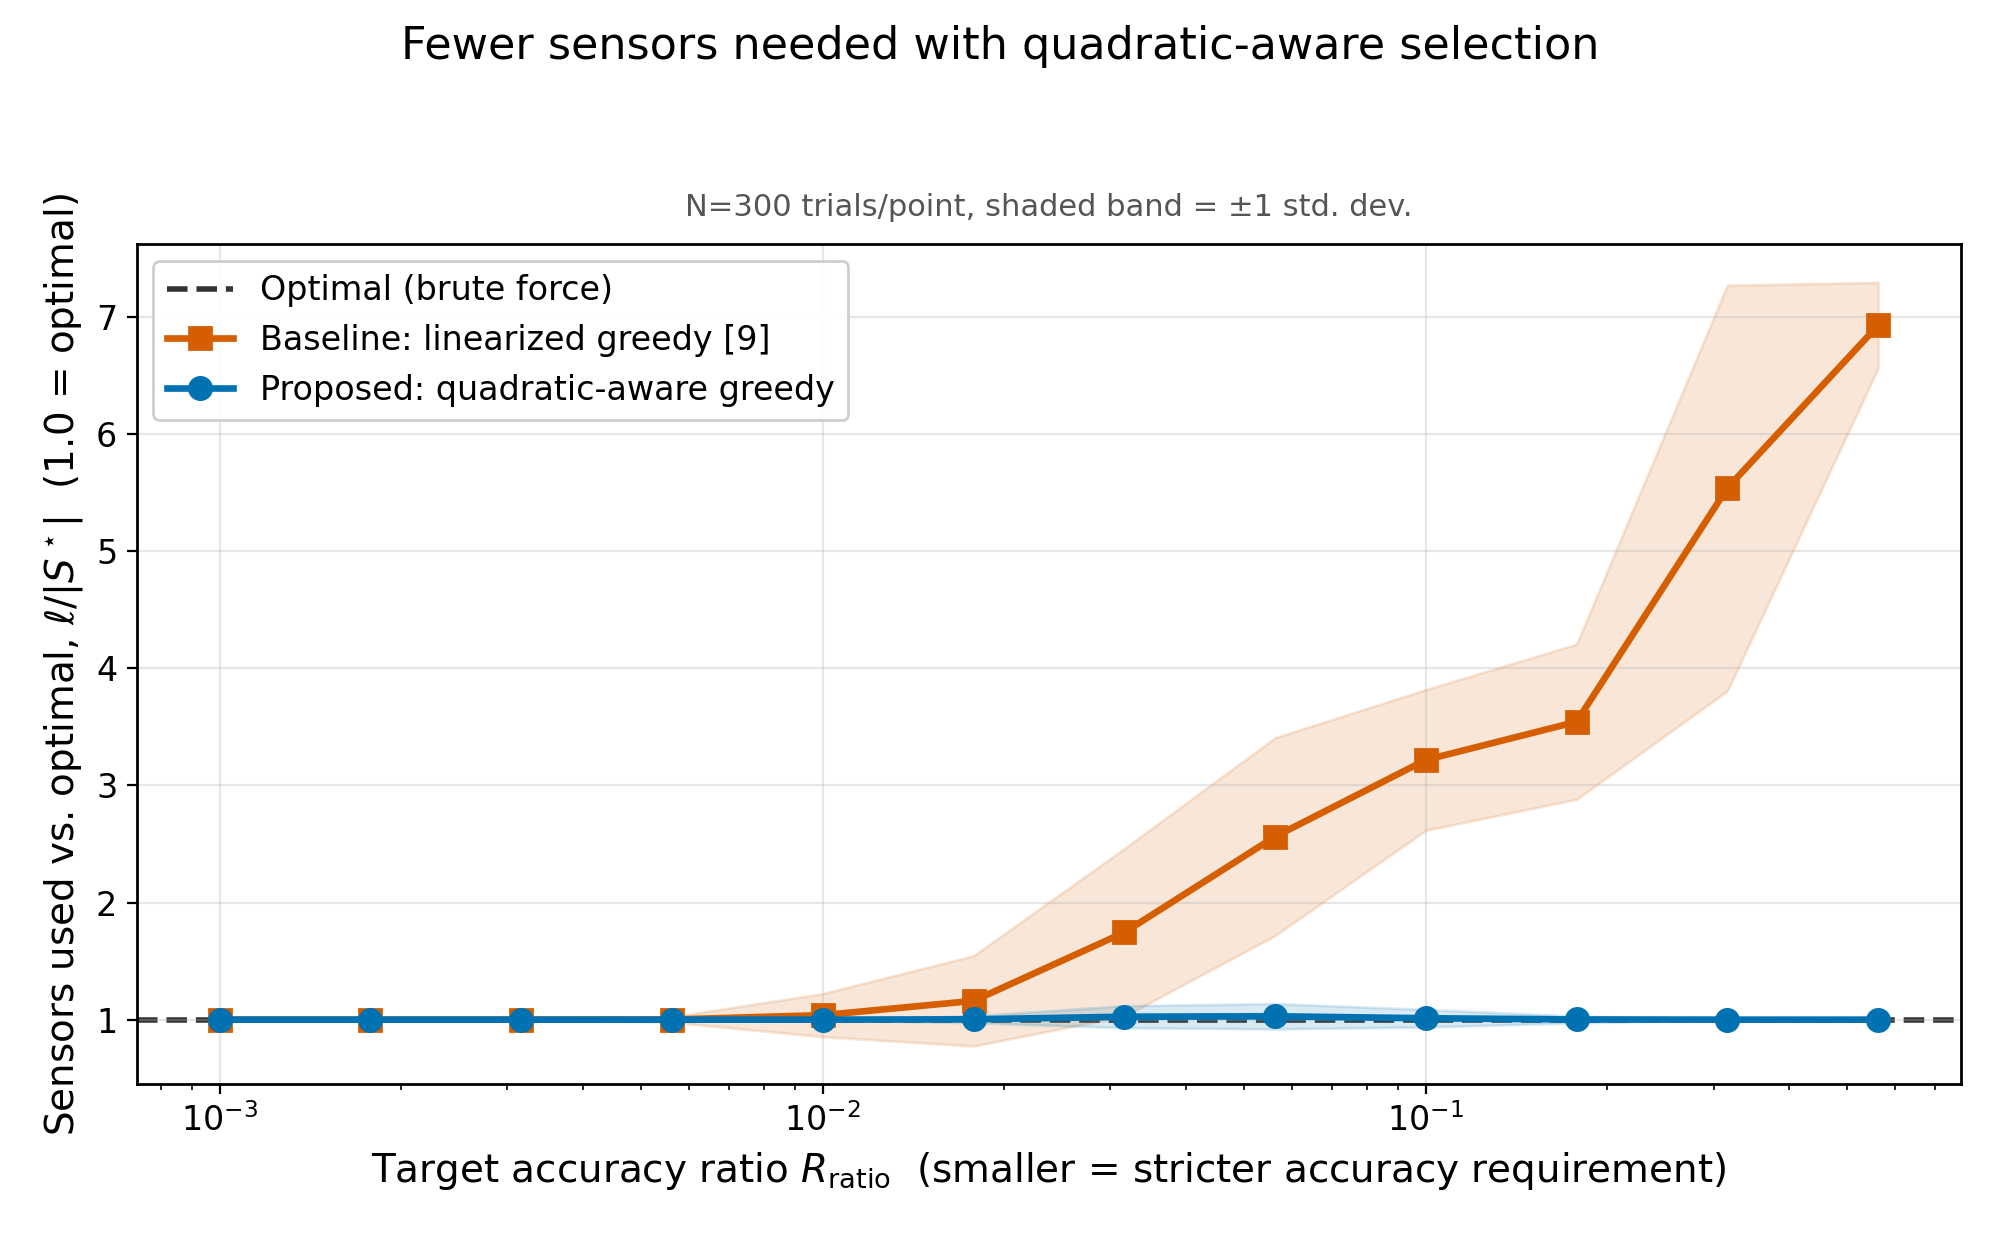
\includegraphics[width=1.02\linewidth]{sensor_selection_test/perf/fig1.png}
        \label{fig:subfig1}
    \end{subfigure}
    \vspace*{-6mm}
    \caption{\small Sensor utilization ratio versus target accuracy ratio. (Orange-red) mean and variance by the linearized greedy baseline \cite{c9}. (Blue) Mean and variance by the proposed greedy quadratic model.}
    \label{fig:mainfig}
\end{figure}

To evaluate the supermodularity-ratio analysis in Theorem~2, Fig.~2 compares the empirical supermodularity ratio with the proposed lower bound under two parameter sweeps using Monte Carlo simulations. Here, we fix $R_{\mathrm{ratio}}=0.01$ and keep the other parameters unchanged. We compute the empirical supermodularity ratio $\gamma_h$ (dark gray), the proposed bound from Theorem~2 (blue), and the bound from~\cite{c19} (orange-red). The plotted curves show the median across valid trials, and the shaded regions indicate the empirical variance range. In the left panel, we vary the scale of the linear measurement term over $[10^{-2}, 10]$ while keeping the other parameters fixed. As the linear-term scale increases, the observation model moves farther from the restrictive pure-quadratic setting considered in previous work. The empirical supermodularity ratio remains above the proposed lower bound across the full sweep, confirming that the proposed bound serves as a valid conservative certificate. Unlike the previous bound, the proposed analysis explicitly captures the effect of the linear term through the $c_j$-dependent terms in the lower-bound expression, and thus remains applicable to the broader mixed linear-quadratic model.



In the right panel, we evaluate the proposed lower bound under a sweep of the measurement-noise scale. We vary the measurement-noise scale over $[10^{0},10^{4}]$ using a fixed nonzero linear-term scale $10$, multiplicated with randomly generated base $C_0$ and the same remaining parameters. The empirical supermodularity ratio stays above both theoretical curves across the full sweep, again confirming that the proposed bound is a valid conservative certificate. The proposed bound is substantially looser than the bound from~\cite{c19} throughout the swept range, and the gap widens rather than narrows as noise increases: roughly three orders of magnitude at $\sigma^2=1$, growing to roughly seven orders of magnitude at $\sigma^2=10^4$. This reflects the conservatism of the per-sensor $\widetilde F_{G,j}$ construction underlying Theorem~2: the pointwise (rather than global) comparator required for the bound to hold for every $\sigma_j^2>0$ comes at the cost of a looser numerical constant, even though the two bounds are not evaluated under matched assumptions -- the~\cite{c19} curve is that reference's own closed-form constant, derived only for rank-one, zero-linear-term sensors, applied here outside its stated range of validity.

\begin{figure}[h]
    \centering
    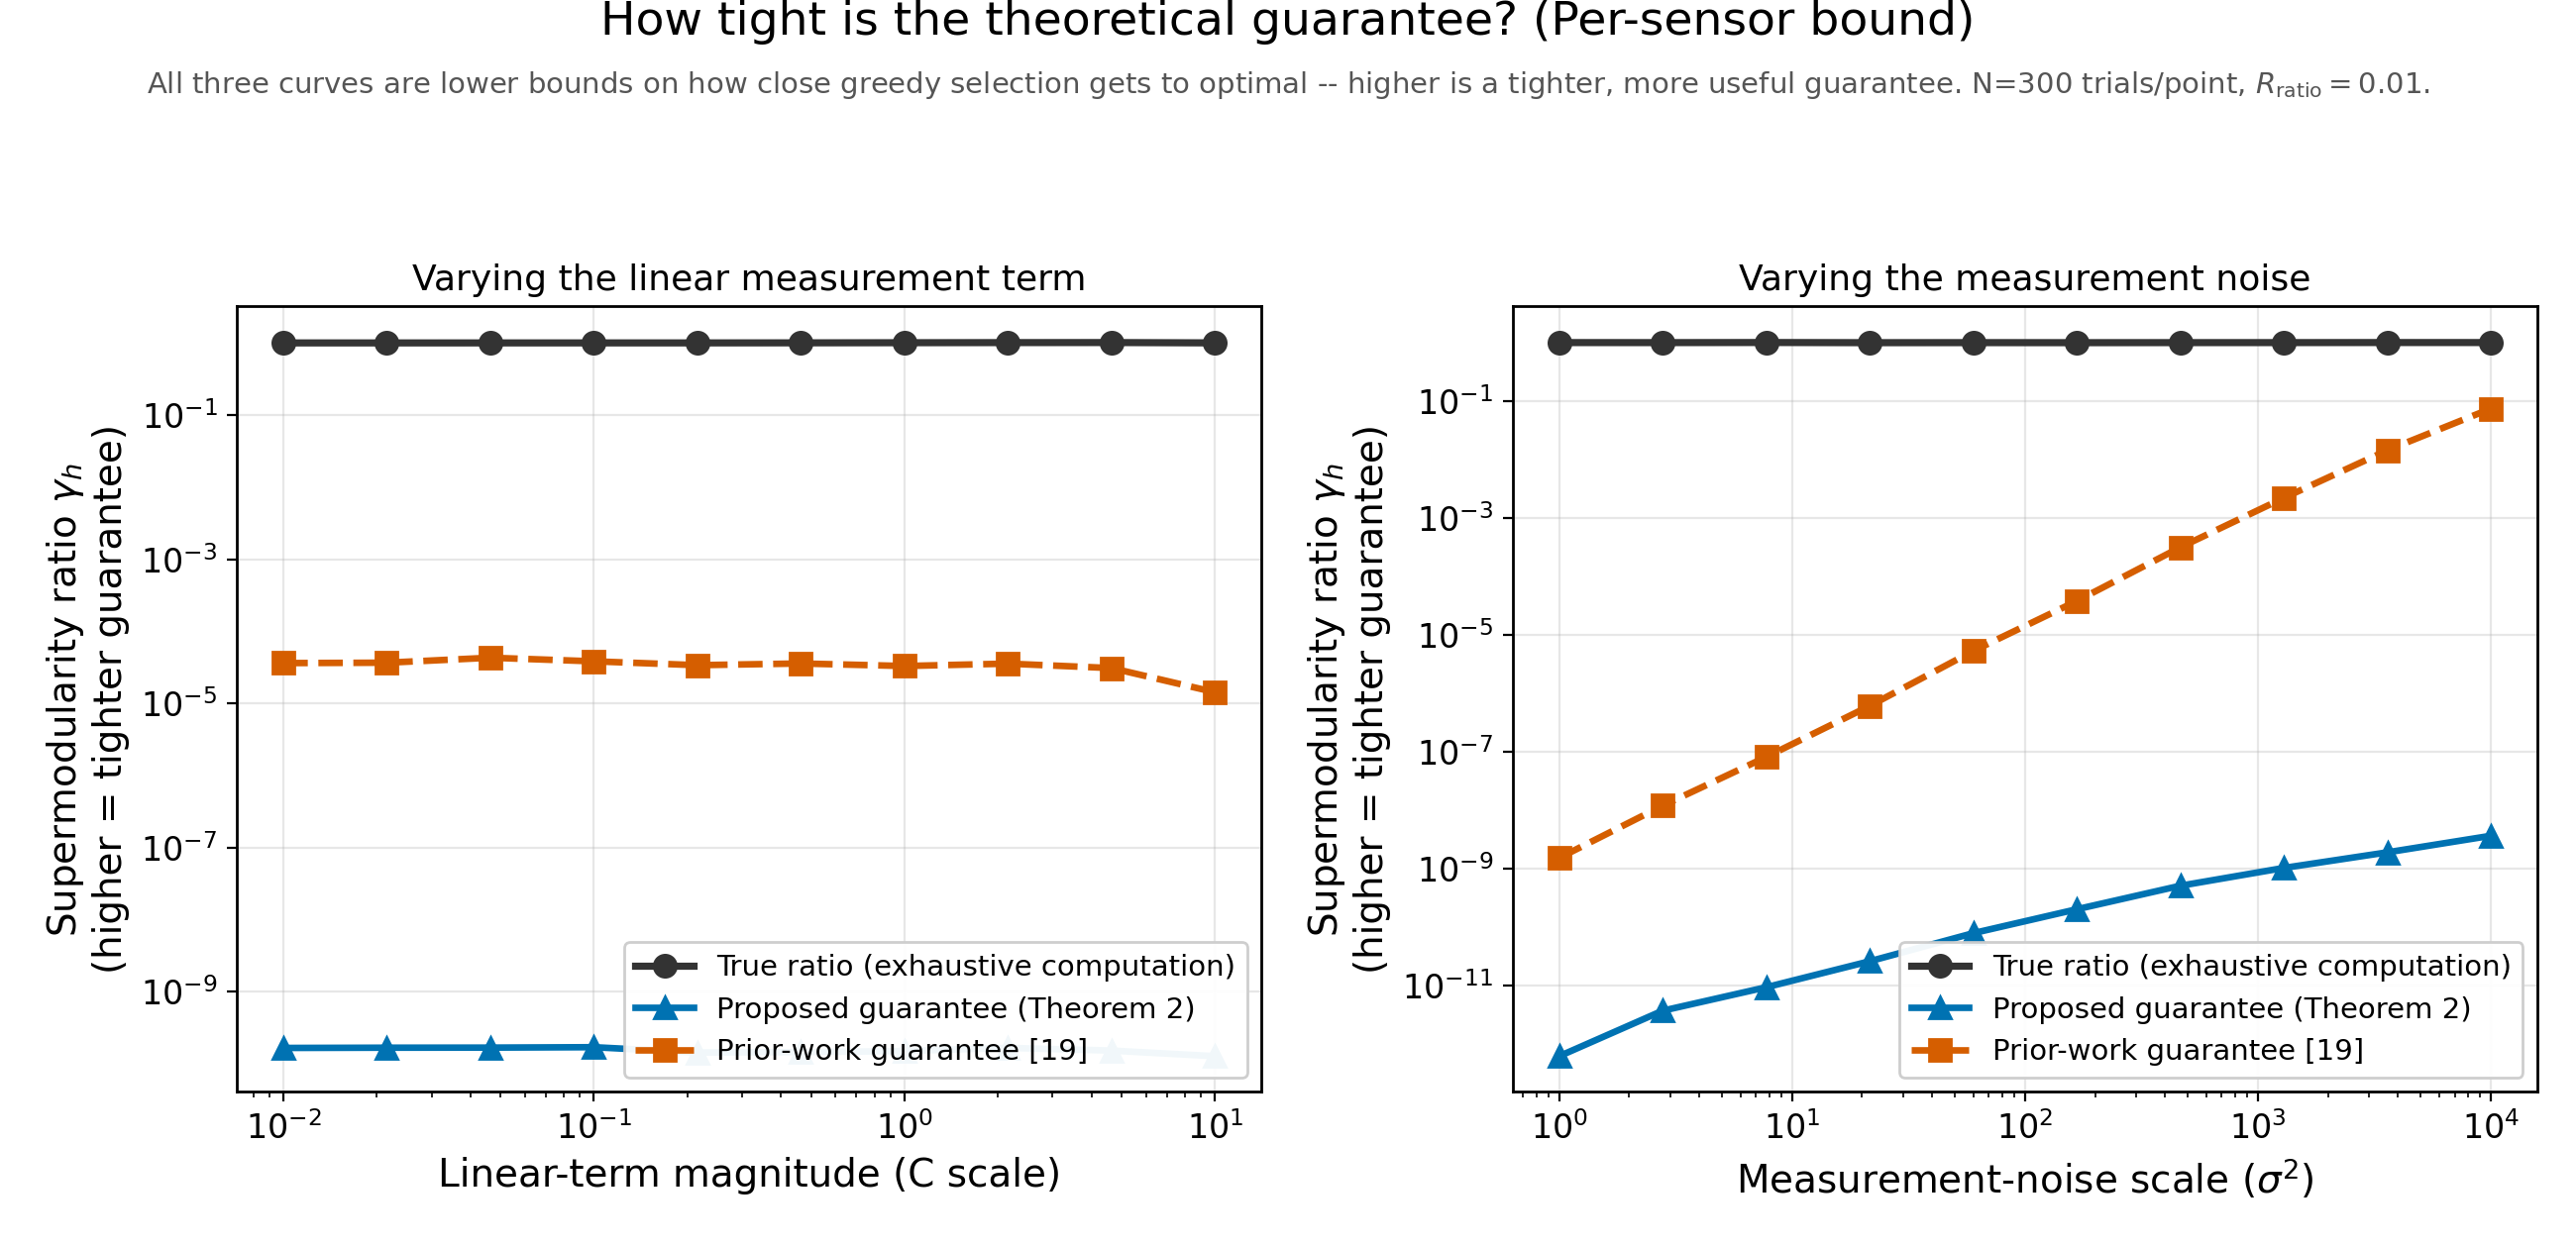
\includegraphics[width=\linewidth]{sensor_selection_test/perf/fig2.png}
    \vspace*{-6mm}
    \caption{\small Empirical supermodularity ratio $\gamma_h$ and theoretical lower bounds under parameter sweeps. (Left): varying the linear-term scale of $C$. (Right): varying the measurement-noise scale $\sigma^2$.}
    \label{fig:supmodfig}
\end{figure}

%Overall, the simulations support both the algorithmic and
%theoretical claims of the paper. Fig.~1 shows that greedy
%selection based on the proposed quadratic objective remains
%close to brute-force optimal in terms of total measurement
%usage, while outperforming a linearization-based
%greedy baseline. Fig.~2 shows that the proposed
%supermodularity-ratio lower bound is numerically valid and
%remains applicable in broader regimes with nonzero linear
%terms. These results show
%that the proposed framework can provide a practically and meaningful analysis for broader applications
%of theoretically grounded approximation for resource-aware
%measurement selection under quadratic observations.

\section{CONCLUSIONS}

%What is the value of your approach beyond this specific solution?

%What is the value of this solution beyond solely solving this subproblem and getting us closer to solving the big picture problem?

We propose a performance-constrained greedy measurement-selection framework for nonlinear quadratic observation models. Using a Van Trees-based A-optimality objective, we establish a measurement-utilization guarantee relative to the optimal measurement usage and derive the first explicit, closed-form lower bound on the supermodularity ratio for sensing models with nonzero linear terms and full-rank quadratic sensing matrices. Unlike previous work, which establishes weak submodularity for this general model only qualitatively and gives an explicit constant only in a restrictive pure-quadratic, rank-1 special case, our bound is explicit and computable for the general model. In future work, we will extend this analysis to time-varying scheduling and other non-submodular estimation metrics.


\addtolength{\textheight}{-12cm}   % This command serves to balance the column lengths
                                  % on the last page of the document manually. It shortens
                                  % the textheight of the last page by a suitable amount.
                                  % This command does not take effect until the next page
                                  % so it should come on the page before the last. Make
                                  % sure that you do not shorten the textheight too much.

%%%%%%%%%%%%%%%%%%%%%%%%%%%%%%%%%%%%%%%%%%%%%%%%%%%%%%%%%%%%%%%%%%%%%%%%%%%%%%%%



%%%%%%%%%%%%%%%%%%%%%%%%%%%%%%%%%%%%%%%%%%%%%%%%%%%%%%%%%%%%%%%%%%%%%%%%%%%%%%%%



%%%%%%%%%%%%%%%%%%%%%%%%%%%%%%%%%%%%%%%%%%%%%%%%%%%%%%%%%%%%%%%%%%%%%%%%%%%%%%%%
%\section*{APPENDIX}

%Appendixes should appear before the acknowledgment.

%\section*{ACKNOWLEDGMENT}

%This work was supported by NASA’s Advanced Information Systems Technology program (Grant No. M2300680). Thank you to Northeastern's Field Robotics Lab for curating an evaluation dataset. %C. H. David was supported by the Jet Propulsion Laboratory, California Institute ofTechnology, under a contract with NASA.



%%%%%%%%%%%%%%%%%%%%%%%%%%%%%%%%%%%%%%%%%%%%%%%%%%%%%%%%%%%%%%%%%%%%%%%%%%%%%%%%

%Reference 

\begin{thebibliography}{99}

\bibitem{c1} Liu, Jun, and Ryan K. Williams. "Optimal intermittent deployment and sensor selection for environmental sensing with multi-robot teams." 2018 IEEE International Conference on Robotics and Automation (ICRA). IEEE, 2018.
\bibitem{c2} Mourikis, Anastasios I., and Stergios I. Roumeliotis. "Optimal sensor scheduling for resource-constrained localization of mobile robot formations." IEEE Transactions on Robotics 22.5 (2006): 917-931.
\bibitem{c3} Golovin, Daniel, Matthew Faulkner, and Andreas Krause. "Online distributed sensor selection." Proceedings of the 9th ACM/IEEE International Conference on Information Processing in Sensor Networks. 2010.
\bibitem{c4} Thatte, Gautam, and Urbashi Mitra. "Sensor selection and power allocation for distributed estimation in sensor networks: Beyond the star topology." IEEE Transactions on Signal Processing 56.7 (2008): 2649-2661.
\bibitem{c5} Lovisari, Enrico, Carlos Canudas de Wit, and Alain Y. Kibangou. "Optimal sensor placement in road transportation networks using virtual variances." 2015 54th IEEE Conference on Decision and Control (CDC). IEEE, 2015.
\bibitem{c6} He, Ying, and K. P. Chong. "Sensor scheduling for target tracking in sensor networks." 2004 43rd IEEE Conference on Decision and Control (CDC)(IEEE Cat. No. 04CH37601). Vol. 1. IEEE, 2004.
\bibitem{c7} Cao, Nianxia, et al. "Sensor selection for target tracking in wireless sensor networks with uncertainty." IEEE Transactions on signal Processing 64.20 (2016): 5191-5204.
\bibitem{c8} Subramanian, Ramanan, and Faramarz Fekri. "Sleep scheduling and lifetime maximization in sensor networks: fundamental limits and optimal solutions." Proceedings of the 5th international conference on Information processing in sensor networks. 2006.
\bibitem{c9} Tzoumas, Vasileios, Ali Jadbabaie, and George J. Pappas. "Sensor placement for optimal Kalman filtering: Fundamental limits, submodularity, and algorithms." 2016 American control conference (ACC). IEEE, 2016.
\bibitem{c10} Zhang, Haotian, Raid Ayoub, and Shreyas Sundaram. "Sensor selection for Kalman filtering of linear dynamical systems: Complexity, limitations and greedy algorithms." Automatica 78 (2017): 202-210.
\bibitem{c11} Ye, Lintao, Sandip Roy, and Shreyas Sundaram. "On the complexity and approximability of optimal sensor selection for Kalman filtering." 2018 Annual American Control Conference (ACC). IEEE, 2018.
\bibitem{c12} Shamaiah, Manohar, Siddhartha Banerjee, and Haris Vikalo. "Greedy sensor selection: Leveraging submodularity." 49th IEEE conference on decision and control (CDC). IEEE, 2010.
\bibitem{c13} Nemhauser, George L., Laurence A. Wolsey, and Marshall L. Fisher. "An analysis of approximations for maximizing submodular set functions—I." Mathematical programming 14 (1978): 265-294.
\bibitem{c14} Fisher, Marshall L., George L. Nemhauser, and Laurence A. Wolsey. "An analysis of approximations for maximizing submodular set functions—II." Polyhedral Combinatorics: Dedicated to the memory of DR Fulkerson. Berlin, Heidelberg: Springer Berlin Heidelberg, 2009. 73-87.
\bibitem{c15} Tzoumas, Vasileios, et al. "LQG control and sensing co-design." IEEE Transactions on Automatic Control 66.4 (2020): 1468-1483.
\bibitem{c16} Summers, Tyler H., Fabrizio L. Cortesi, and John Lygeros. "On submodularity and controllability in complex dynamical networks." IEEE Transactions on Control of Network Systems 3.1 (2015): 91-101.
\bibitem{c17} Shen, Xiaojing, Sijia Liu, and Pramod K. Varshney. "Sensor selection for nonlinear systems in large sensor networks." IEEE Transactions on Aerospace and Electronic Systems 50.4 (2014): 2664-2678.
\bibitem{c18} Haber, Aleksandar, Ferenc Molnar, and Adilson E. Motter. "State observation and sensor selection for nonlinear networks." IEEE Transactions on Control of Network Systems 5.2 (2017): 694-708.
%\bibitem{c12} Yang, Chun, Lance Kaplan, and Erik Blasch. "Performance measures of covariance and information matrices in resource management for target state estimation." IEEE Transactions on Aerospace and Electronic Systems 48.3 (2012): 2594-2613.
\bibitem{c19} Hashemi, Abolfazl, et al. "Submodular observation selection and information gathering for quadratic models." International Conference on Machine Learning. PMLR, 2019.
\bibitem{c20} Hashemi, Abolfazl, et al. "Supplementary material for “Submodular Observation Selection and Information Gathering for Quadratic Models”."
\bibitem{c21} Van Trees, Harry L., and Kristine L. Bell. Detection estimation and modulation theory, part I: detection, estimation, and filtering theory. John Wiley & Sons, 2013.
\bibitem{c22} Krause, Andreas, and Carlos Guestrin. "A note on the budgeted maximization of submodular functions." (2005): 103.
\bibitem{c23} Wolsey, Laurence A. "An analysis of the greedy algorithm for the submodular set covering problem." Combinatorica 2.4 (1982): 385-393.
\bibitem{c24} Horn, Roger A., and Charles R. Johnson. Matrix Analysis. 2nd ed. Cambridge University Press, 2012.
\bibitem{c25} Woodbury, Max A. "Inverting modified matrices." Memorandum Report 42, Statistical Research Group, Princeton University, 1950.
\bibitem{c26} Das, Abhimanyu, and David Kempe. "Submodular meets spectral: Greedy algorithms for subset selection, sparse approximation and dictionary selection." International Conference on Machine Learning. 2011.
\end{thebibliography}

%Performance_Measures_of_Covariance_and_Information_Matrices_in_Resource_Management_for_Target_State_Estimation


\end{document}
